\documentclass[a4paper]{article}
\usepackage[pdftex]{graphicx}
\usepackage[utf8]{inputenc}
\usepackage{enumerate}
\usepackage{siunitx}
\sisetup{locale=DE} 
\usepackage{icomma}
\usepackage{amssymb}
\usepackage{tikz}
\usepackage{href-ul}
\hypersetup{
	colorlinks=true,
	linkcolor=blue,
	urlcolor=blue}
\usepackage{geometry}
\geometry{a4paper, top=15mm, left=15mm, right=15mm, bottom=15mm,
	headsep=10mm, footskip=12mm}


\begin{document}
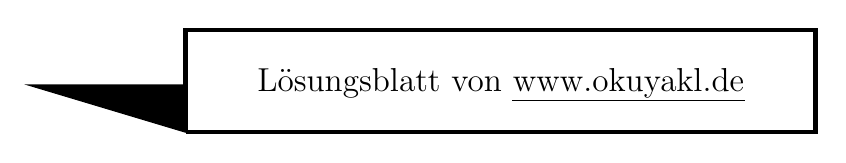
\begin{tikzpicture}(10,3)
	\draw[ultra thick](2,0) --(10,0) -- (10,1.3) --(2,1.3) -- (2,0);
	\draw[fill=black](2,0)-- (0,.6) -- (2,.6) -- (2,0);
	\node at (6,.6) {\large Lösungsblatt von \href{https://www.okuyakl.de}{www.okuyakl.de}};
\end{tikzpicture}
\vspace{0.5 cm}

\noindent {\bf Aufgabe 1.a)}\\
\begin{minipage}{0.3\textwidth}
In der Skizze ist $d$ der zu berechnende Spaltabstand $a={\SI{17,6}{\centi\meter}\over 2}=\SI{8,8}{\centi\meter}$ der Abstand des ersten Maximums zur Schirmmitte und $l=\SI{2,80}{\meter}$ der Abstand des Schirms zum Doppelspalt.
\end{minipage}
\begin{minipage}{0.7\textwidth}
\includegraphics[width=10 cm]{beu95.pdf}
\end{minipage}

Aus der Geometrie dieser Anordnung folgt näherungsweise für kleine Winkel:
$$ 
\renewcommand{\arraystretch}{2}
\begin{array}{rcl}
{\lambda \over d} &\approx& {a\over l} \quad (*)\\
d &=&  {l \over a} \cdot \lambda \\
d &=&  {\SI{2,80}{\meter} \over \SI{0,088}{\meter}}\cdot\SI{546e-9}{\meter}\\
d &=& \SI{17e-6}{\meter} = 17\SI{}{\micro\meter} 
\end{array}
$$

Der Spaltabstand beträgt somit $\SI{17}{\micro\meter}$.
\vspace{0.5 cm}

\noindent {\bf Aufgabe 1.b)}\\
Nach $(*)$ gilt $a \sim \lambda$. Damit verringert sich mit der Wellenlänge auch der Abstand der Intensitätsmaxima auf dem Schirm.  Die Anzahl der beobachtbaren Maxima muss somit zunehmen.
\vspace{0.5 cm}

\noindent{\bf Aufgabe 2.}\\
Wir subtrahieren die beiden Gleichungen und lösen nach l auf:
$$
\renewcommand{\arraystretch}{2}
\begin{array}{rcll}
{\lambda_1 \over d} &=& {a_1\over l}\\
{\lambda_2 \over d} &=& {a_2\over l}\\
\hline
{\lambda_1 -\lambda_2 \over d} &=& {a_1-a_2 \over l}\\
l &=& {(a_1-a_2)} \cdot {d \over \lambda_1 -\lambda_2}\\
l &=& {\SI{0,003}{\meter}\cdot\SI{1e-4}{\meter}  \over \SI{5,8959e-7}{\meter}-\SI{5,8899e-7}{\meter}}\\
l&=& \SI{500}{\meter}
\end{array}
$$
Die Natrium-Doppellinie lässt sich mit dieser Anordnung nicht auftrennen.
\vspace{0.5 cm}

\begin{center}
	\includegraphics[width=7 cm]{../../viecher/endcomic.pdf}
	
	Hier geht es zurück zum \href{https://www.okuyakl.de/phys/p11wellL095/aa095.pdf}{Aufgabenblatt}
\end{center}


%Ende
\end{document}
